\subsection{Mediciones}

Para analizar el comportamiento del algoritmo, medimos el tiempo de ejecución para distintos tamaños de entrada. Luego, con los tiempos obtenidos, realizamos un ajuste por cuadrados mínimos utilizando una función lineal de la forma:

\[
T(n) = c_1n + c_2
\]

Elegimos este modelo porque, según el análisis teórico realizado anteriormente, el algoritmo tiene complejidad temporal $O(n)$. Por lo tanto, se espera que el tiempo de ejecución aumente aproximadamente de forma lineal con el tamaño de la entrada.

\subsubsection{Generación de los conjuntos de datos}

Para realizar las mediciones se generaron conjuntos de datos de distintos tamaños. Cada conjunto representa una fila de monedas, cuyos valores son enteros generados aleatoriamente entre 1 y 1000 inclusive. Los valores se guardaron en el mismo orden en que fueron generados y separados por ``;''.

Los tamaños utilizados fueron:

\[
20,\ 25,\ 50,\ 100,\ 500,\ 1000,\ 5000,\ 10000,\ 20000,\ 50000,
\]
\[
100000,\ 200000,\ 500000,\ 1000000,\ 2000000,\ 5000000,\ 7500000,\ 10000000.
\]

\newpage
\subsubsection{Metodología de medición}

Para cada tamaño de entrada se realizaron cinco ejecuciones del algoritmo y se registró el tiempo de cada una. Luego, se calculó el promedio:

\[
T(n) = \frac{1}{5}\sum_{i=1}^{5} T_i(n)
\]

De esta forma, se utilizó el promedio como el tiempo representativo para cada tamaño de entrada, reduciendo el efecto de posibles variaciones entre ejecuciones.

A partir de los tiempos obtenidos se realizó un ajuste por cuadrados mínimos utilizando la función:

\[
\hat{T}(n) = c_1n + c_2
\]

Los valores de $c_1$ y $c_2$ se obtuvieron minimizando el error cuadrático entre los tiempos medidos y los tiempos dados por el ajuste.

\begin{figure}[H]
    \centering
    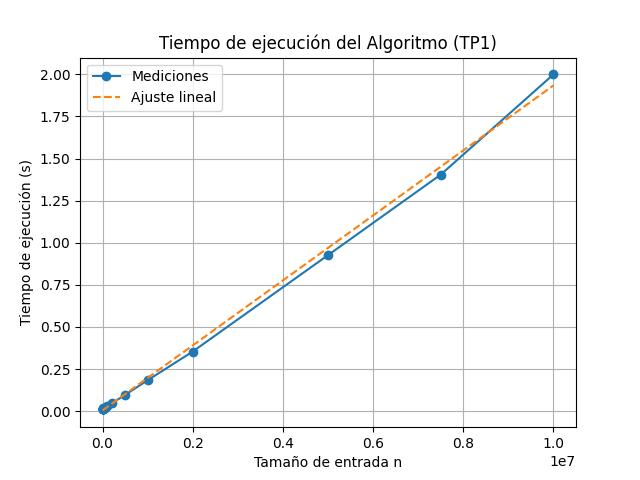
\includegraphics[width=0.9\textwidth]{img/tiempo_ajuste.png}
    \caption{Tiempo de ejecución en función del tamaño de entrada y ajuste lineal.}
    \label{fig:tiempo}
\end{figure}

En la Figura~\ref{fig:tiempo} se puede observar que los tiempos presentan una tendencia aproximadamente lineal a medida que aumenta el tamaño de la entrada. Esto coincide con la complejidad $O(n)$ obtenida en el análisis teórico.

\subsubsection{Error absoluto}

Para observar qué tan bien se ajusta la función lineal a las mediciones, se calculó el error absoluto para cada tamaño de entrada:

\[
E(n) = \left|T(n) - \hat{T}(n)\right|
\]

donde $T(n)$ es el tiempo medido y $\hat{T}(n)$ es el tiempo estimado por el ajuste lineal.

\begin{figure}[H]
    \centering
    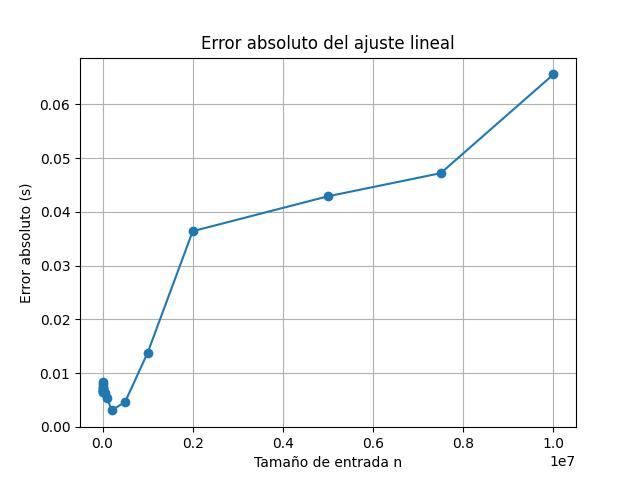
\includegraphics[width=0.9\textwidth]{img/error_ajuste.png}
    \caption{Error absoluto del ajuste lineal para cada tamaño de entrada.}
    \label{fig:error}
\end{figure}

La Figura~\ref{fig:error} muestra la diferencia entre los tiempos medidos y los estimados por el modelo. El error puede variar debido a factores externos a la ejecución del algoritmo, como la carga del sistema o el tiempo necesario para leer los archivos de entrada.
